\documentclass[report.tex]{subfiles}

\begin{document}
\section{Finite Element Modelling}
The FEM simulations were run using the Object Oriented Finite (OOF) element analysis program called OOF2, created by the National Institute of Standards and Technology (available here: \url{https://www.ctcms.nist.gov/oof/oof2/}) \cite{OOF2Modelling}. Minor changes to the simulation were altered in the Python code, rather than using the OOF2 graphical user interface (GUI) as this saved time. Four test cases were trialed to ensure the simulation was generating results as expected, the simplest case is heat diffusion through a simple shape and the most complex incorporating heat diffusion and displacement in a single grain of Ti-6Al-4V. Once the test cases proved successful, the FEM simulation was run for a larger section of Ti-6Al-4V and the heat diffusion and displacement were determined.

\subsection{Model Validation}
The first test case is a simple star shape, test cases 2-4 are all Ti-6Al-4V (Figure \ref{fig:OOF2Input}).
\\
\begin{figure}[h]
    \centering
    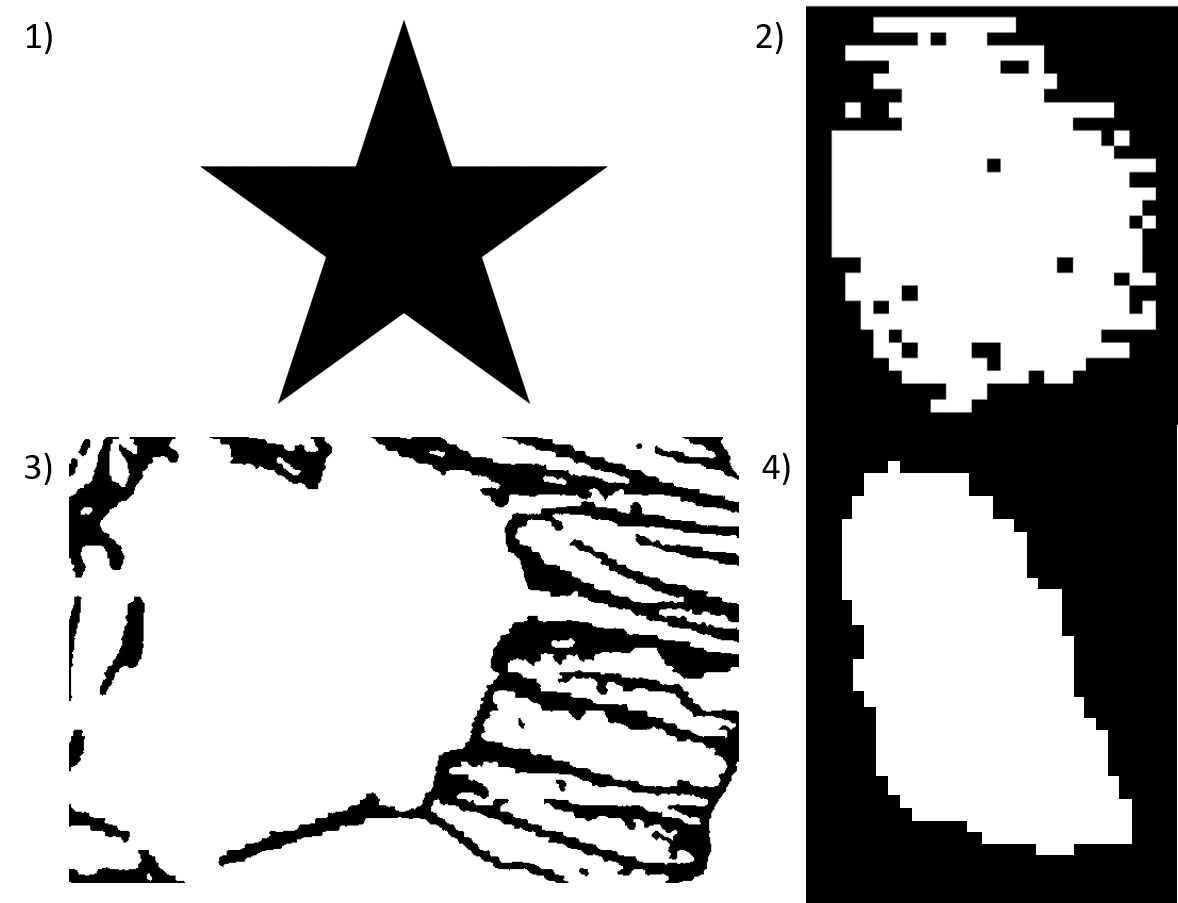
\includegraphics[width=10cm]{Model Validation Input Images.png}
    \caption{OOF2 input files for the test cases}
    \label{fig:OOF2Input}
\end{figure}
\\
Each test case input was a binary file, where the black and white regions are specified as separate materials. The thermo-physical properties of the black and white regions are assigned as specified in Table \ref{tab:validation}: Young's Modulus, \textit{E}, Poisson's Ratio, $\nu$, thermal conductivity, $\kappa$, and thermal expansion coefficient, $\alpha$. The microstructure skeleton is created using a 40x40 QuadSkeleton grid, which is annealed, the edges are swapped and the skeleton smoothed to improve the homogeneity index (shown Table \ref{tab:validation}). The mesh is then generated from the skeleton, with the mapping and interpolation orders remain as 1 to save on computational time. The fields are then defined in accordance to Table \ref{tab:validation} on the mesh, constrained in-plane as active (such that the FE output contains the specified parameters). The boundary conditions are set as 0 \degree C on the left edge and 1000 \degree C on the right edge. When the force field is applied, the left edge displacement in (x,y) is fixed at (0,0). The solver tolerance is set to 1 x10$^-^1^3$ with 1000 iterations and the results are visualised. For test case 4, the stress contour map is created in post processing within the OOF2 program where the flux is set to stress and the invariant is set to trace.

\begin{center}
  \begin{table}[t!]
  \caption{\label{tab:validation}Physical Properties, Homogeneity Index, Model Fields and Boundary Conditions of Test Cases 1-4}

  \begin{tabular}{|p{1cm}|p{3cm}|p{3cm}|p{2.5cm}|p{2.2cm}|p{2.5cm}|}
  \hline
  \centering
  \textbf{Test Case} &\textbf{Black Region Properties} &\textbf{White Region Properties} &\textbf{Homogeneity Index} &\textbf{Fields} &\textbf{Boundary Conditions}\\
  \hline
   1 & E = 300 GPa \newline $\nu$ = 0.33 \newline $\kappa$ = 1000 W/mK \newline $\alpha$ = 5 x10$^-^6$ K$^-^1$ & E = 10 GPa \newline $\nu$ = 0.27 \newline $\kappa$ = 1 W/mK \newline $\alpha$ = 1 K$^-^1$ & 0.992 & Temperature & 0 - 1000 \degree C \\
   \hline
   2 & E = 117 GPa \newline $\nu$ = 0.33 \newline $\kappa$ = 390 W/mK \newline $\alpha$ = 51 x10$^-^6$ K$^-^1$ & E = 200 GPa \newline $\nu$ = 0.27 \newline $\kappa$ = 41 W/mK \newline $\alpha$ = 36 K$^-^1$ & 0.996 & Temperature \newline Force & 0 - 1000 \degree C \newline Left side (x,y) fixed at (0,0) \\
   \hline
   3 & E = 150 GPa \newline $\nu$ = 0.33 \newline $\kappa$ = 8.5 W/mK \newline $\alpha$ = 10 x10$^-^6$ K$^-^1$ & E = 117 GPa \newline $\nu$ = 0.34 \newline $\kappa$ = 6.7 W/mK \newline $\alpha$ = 8.6 x10$^-^6$ K$^-^1$ & 0.958 & Temperature \newline Force & 0 - 1000 \degree C \newline Left side (x,y) fixed at (0,0) \\
   \hline
   4 & E = 40 GPa \newline $\nu$ = 0.33 \newline $\kappa$ = 15 W/mK \newline $\alpha$ = 1 x10$^-^3$ K$^-^1$ & E = 117 GPa \newline $\nu$ = 0.34 \newline $\kappa$ = 6.7 W/mK \newline $\alpha$ = 8.6 x10$^-^6$ K$^-^1$ & 0.995 & Temperature \newline Force & 0 - 1000 \degree C \newline Left side (x,y) fixed at (0,0) \\ 
   \hline
  \end{tabular}
  \end{table}
\end{center}
\\
The results from test case 1 are shown in figure \ref{fig:TestCase1Results} and clearly show the heat diffusion through the star shape. The properties assigned to the image, where the black region conducts the heat more effectively than the white region, can clearly be seen in the heat profile. The thermal gradient is much more steady when the heat flows through a white region compared to the longest cross-section of the black star shape, which remains at approximately 400 - 500 \degree C from point to point. These results suggest the simulation is working correctly and so, the simulation can be made more complex with the inclusion of the force field.
\\
\begin{figure}[h]
    \centering
    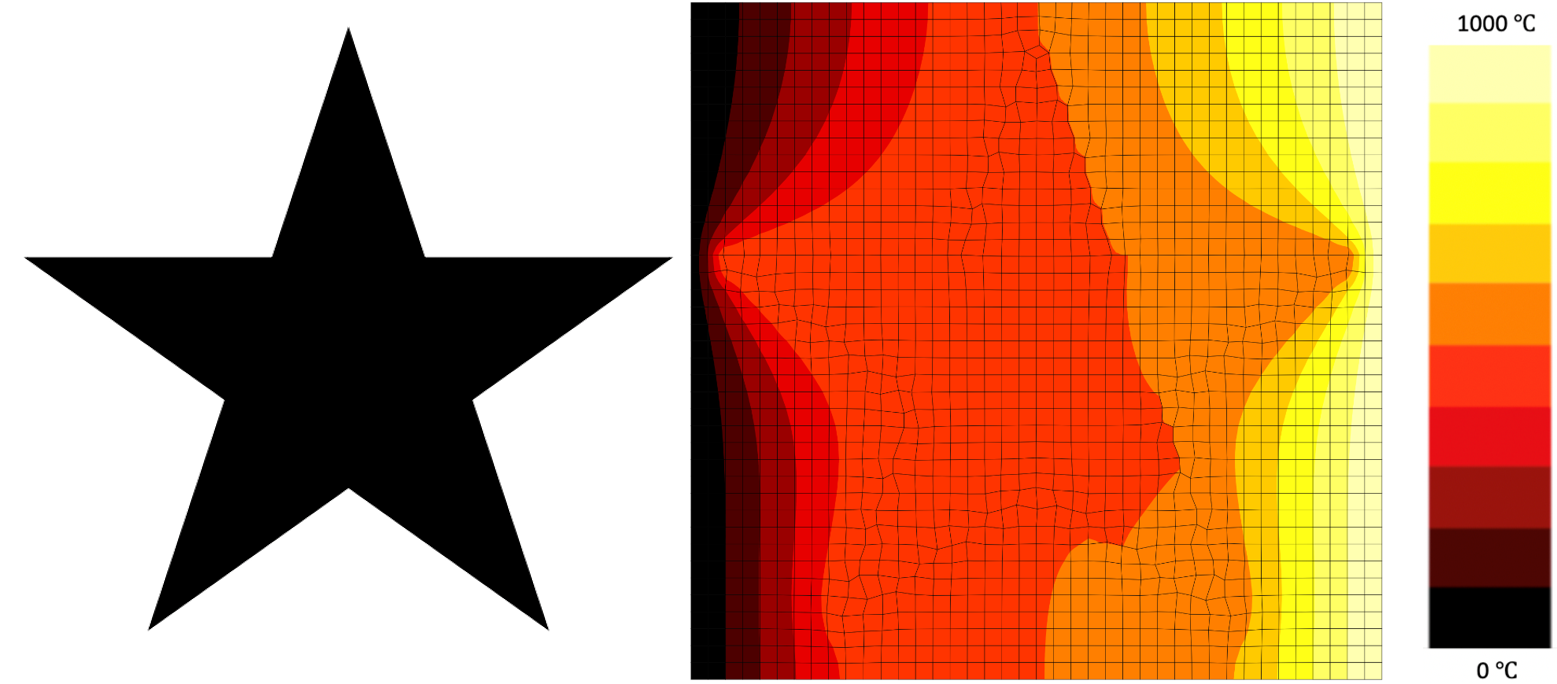
\includegraphics[width=14cm]{TestCase1_Simulation_Results_Corrected.png}
    \caption{Test case 1 results, showing the original input file and the heat diffusion through the star shape}
    \label{fig:TestCase1Results}
\end{figure}
\\
The simulation run for test case 2 involved the temperature and force fields in the OOF2 GUI, and the results are shown in figure \ref{fig:TestCase2Results}. The material properties used for this simulation are similar to that of the alpha and beta regions of Ti-6Al-4V. The difference in the coefficient of thermal expansion between the regions has caused the displacement which is clearly visible towards the right of the simulation result images, with the displacement range being higher in the y-direction by 5.03 $\micro$m. The difference between the thermal conductivity values assigned to each region is small, so the thermal gradient is relatively consistent across the grain. A more complex structure can be looked at for the next test case.
\\
\begin{figure}[htp]
    \centering
    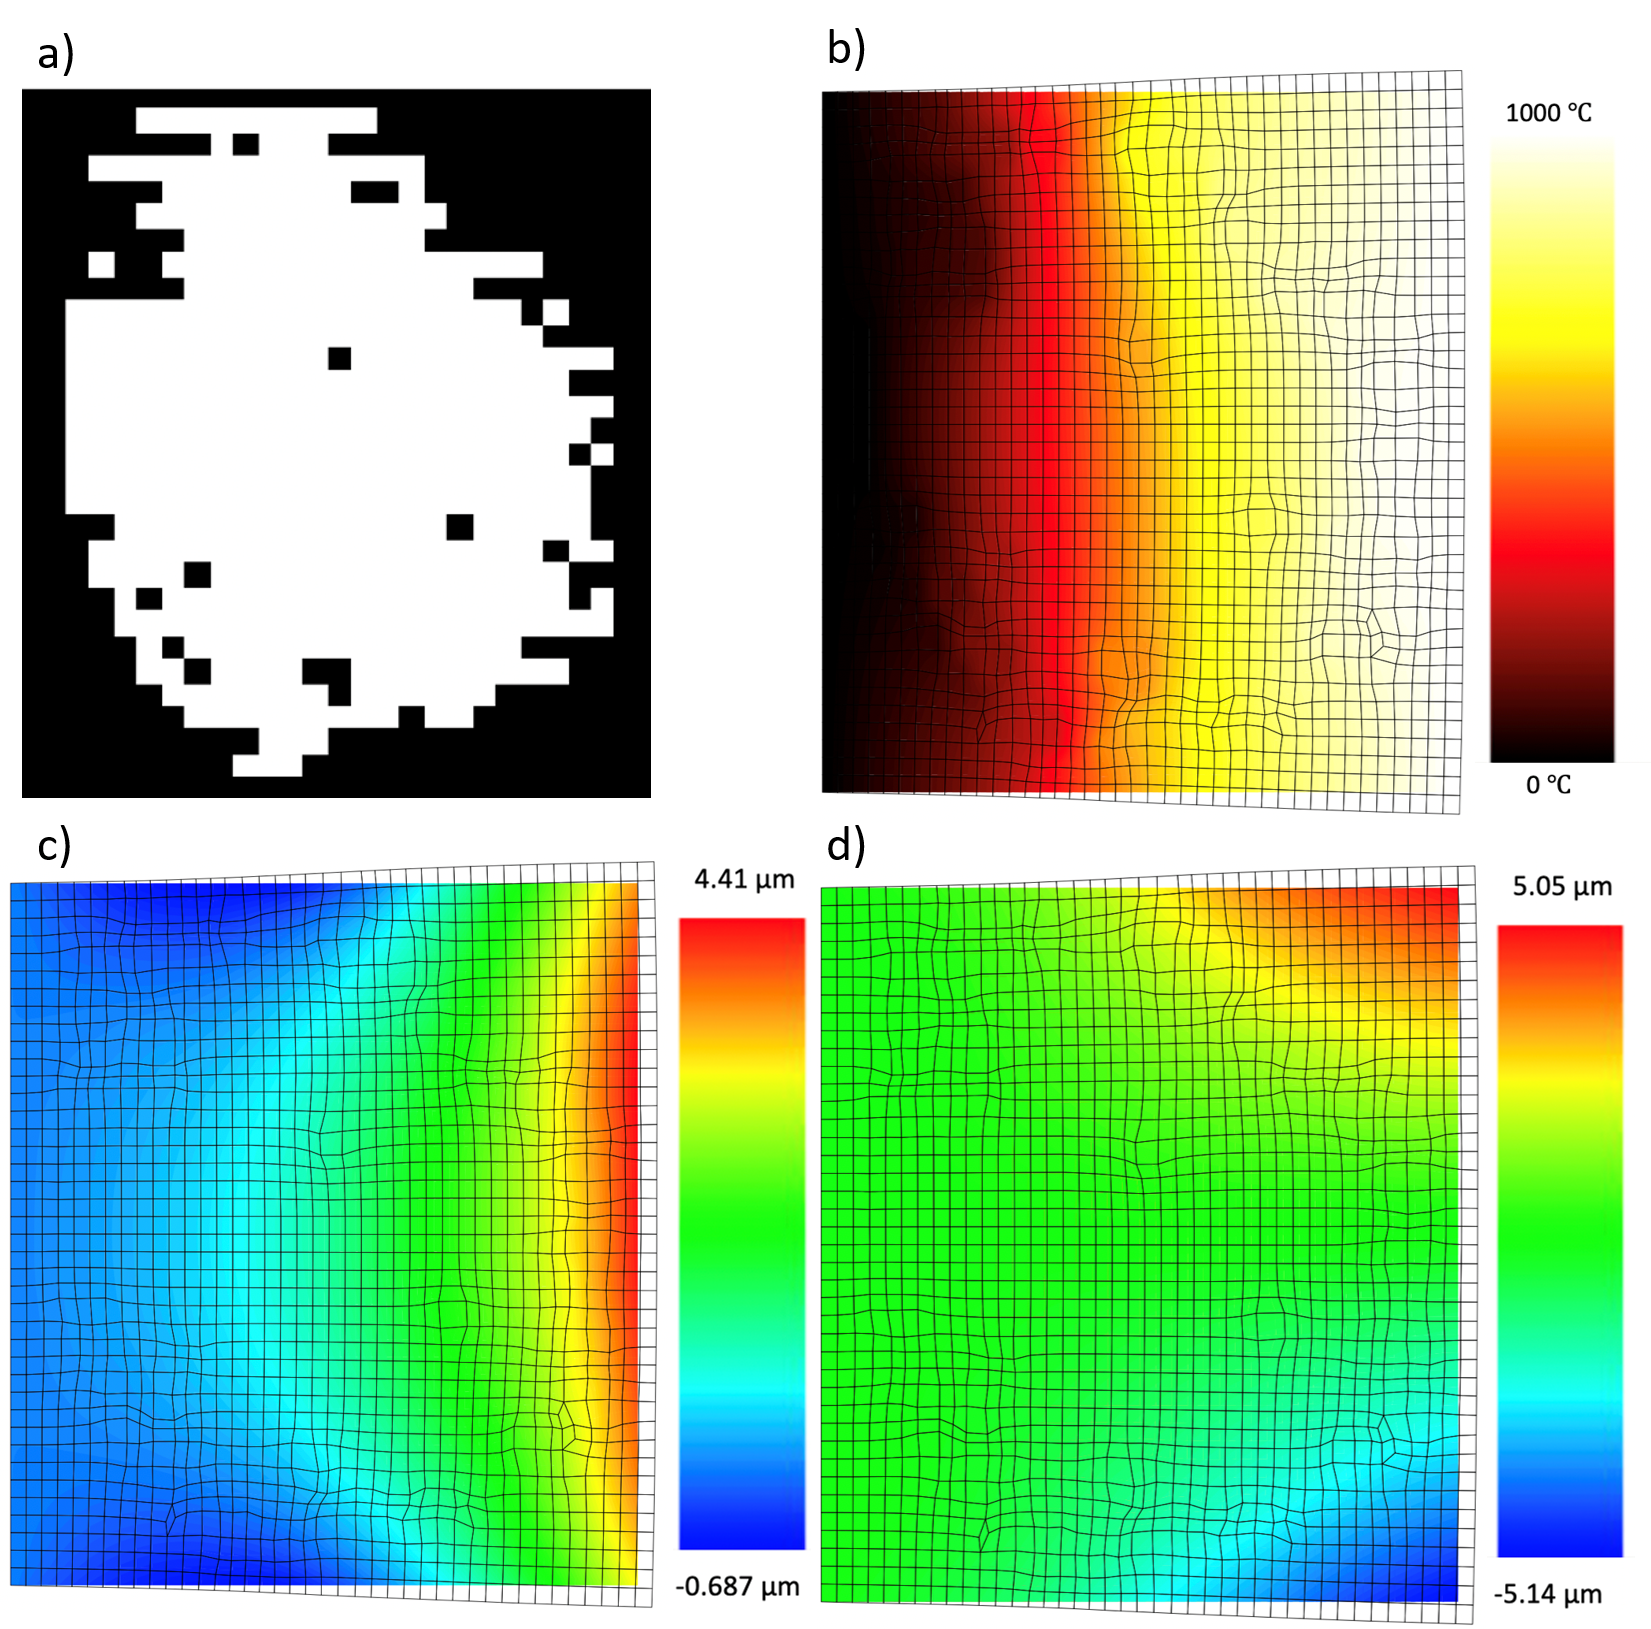
\includegraphics[width=15cm]{TestCase2_Simulation_Results.png}
    \caption{Test case 2 results, showing the a) original microstructure of Ti-6Al-5V b) heat diffusion through the grain c) displacement in the x-direction d) displacement in y-direction}
    \label{fig:TestCase2Results}
\end{figure}
\\
Test case 3 has a binary image of Ti-6Al-4V with multiple grains as the input file, to determine the impact of multiple grain boundaries on the simulation quality. The temperature and displacement contours are shown in figure \ref{fig:TestCase3Results}. The material properties are similar between the black and white regions to simplify the simulation and ensure an output is obtained within a reasonable computational time frame. The results are as expected for a simulation with minor material property variations, with the temperature varying linearly in the x-direction and the displacement being consistent in the x- and y-directions. The inclusion of a stress contour can be examined for the next simulation, as it is clear that multiple grains can be processed in the simulation.
\\
\begin{figure}[htp]
    \centering
    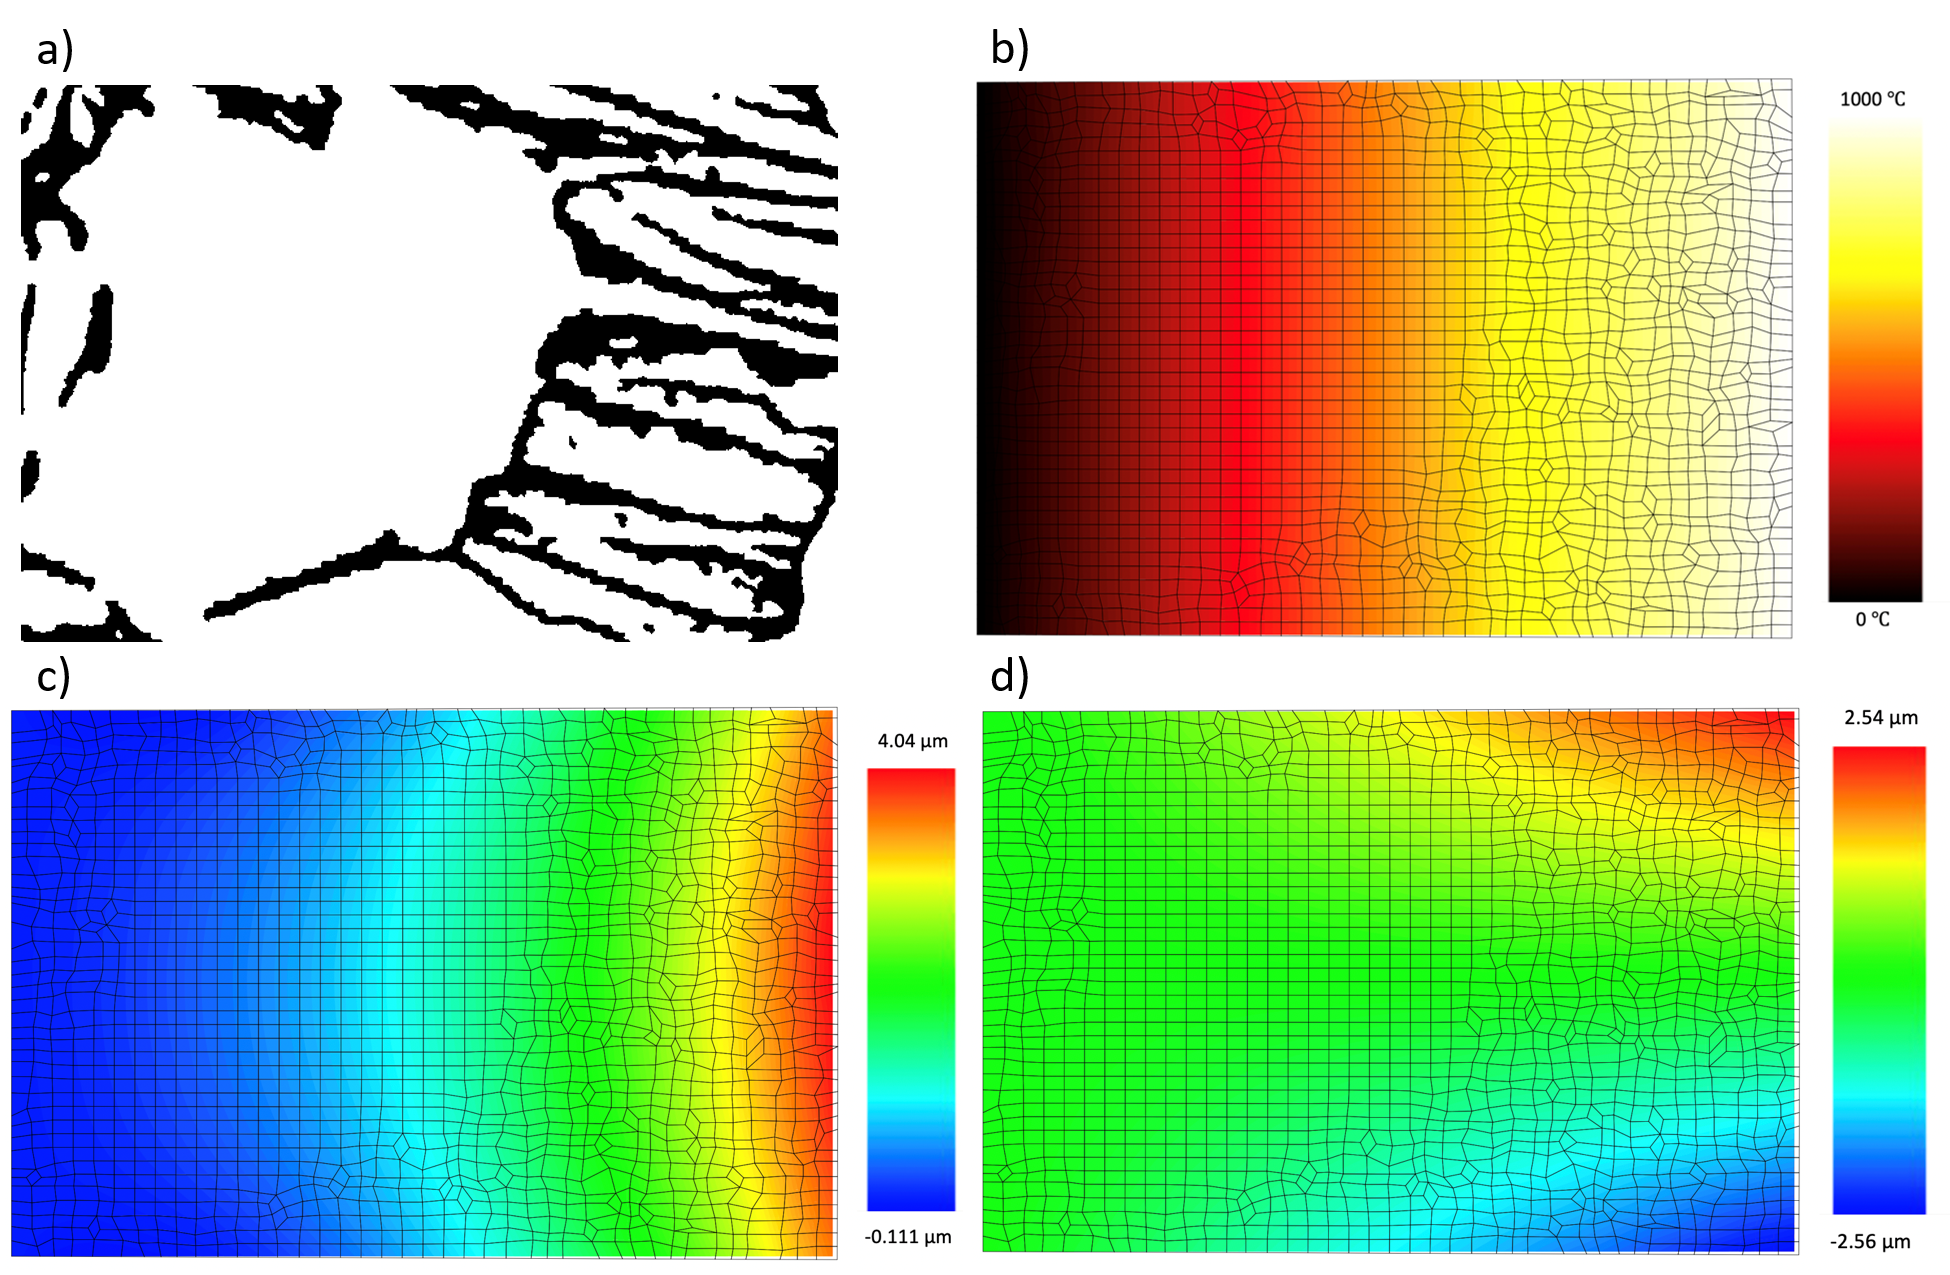
\includegraphics[width=15cm]{TestCase3_Simulation_Results.png}
    \caption{Test case 3 results, showing the a) original microstructure of Ti-6Al-5V b) heat diffusion through the grains c) displacement in the x-direction d) displacement in y-direction}
    \label{fig:TestCase3Results}
\end{figure}
\\
Test case 4 used a binary input of a Ti-6Al-4V grain which was image processed using the method described in the Image Analysis section. The material properties in this simulation were exaggerated to determine the impact on the results and ensure the model holds true for such cases. The large difference in coefficient of thermal expansion between the black and white regions is clear in the visualisation of the mesh over the contour plots shown in figure \ref{fig:TestCase4Results}. The y-displacement totals 40.6 $\micro$m and the x-displacement totals 20.4 $\micro$m, which is significantly larger than the previous tests. The stress map was added as an output for this test case and the result show the most significant stresses were concentrated on the grain boundaries, particularly at higher temperatures, where stresses reached 2.61 x10$^5$ N/m$^2$.\\
\\
The test results have shown that the simulation is able to process binary images with multiple grains to produce contour plots of temperature distribution, displacement along x and y, and stress distribution. This means that the FEM is capable of running the final simulation to gain information about the heat diffusion through a multi-grain Ti-6Al-4V image and the results can be trusted.
\\
\begin{figure}[htp]
    \centering
    \includegraphics[width=15cm]{TestCase4_Simulation_Results.png}
    \caption{Test case 4 results, showing the a) original microstructure of Ti-6Al-5V b) heat diffusion through the grain c) stress within the grain d) displacement in the x-direction e) displacement in y-direction}
    \label{fig:TestCase4Results}
\end{figure}

\clearpage
\subsection{FEM of a Globular Ti-6Al-4V Microstructure}

The FEM is used to simulate heat diffusion, displacement and stress distribution in a binary image of a globular Ti-6Al-4V microstructure \ref{fig:FinalSimulationInput}. Only a section of the original image was used to save on computational time.
\\
\begin{figure}[h!]
    \centering
    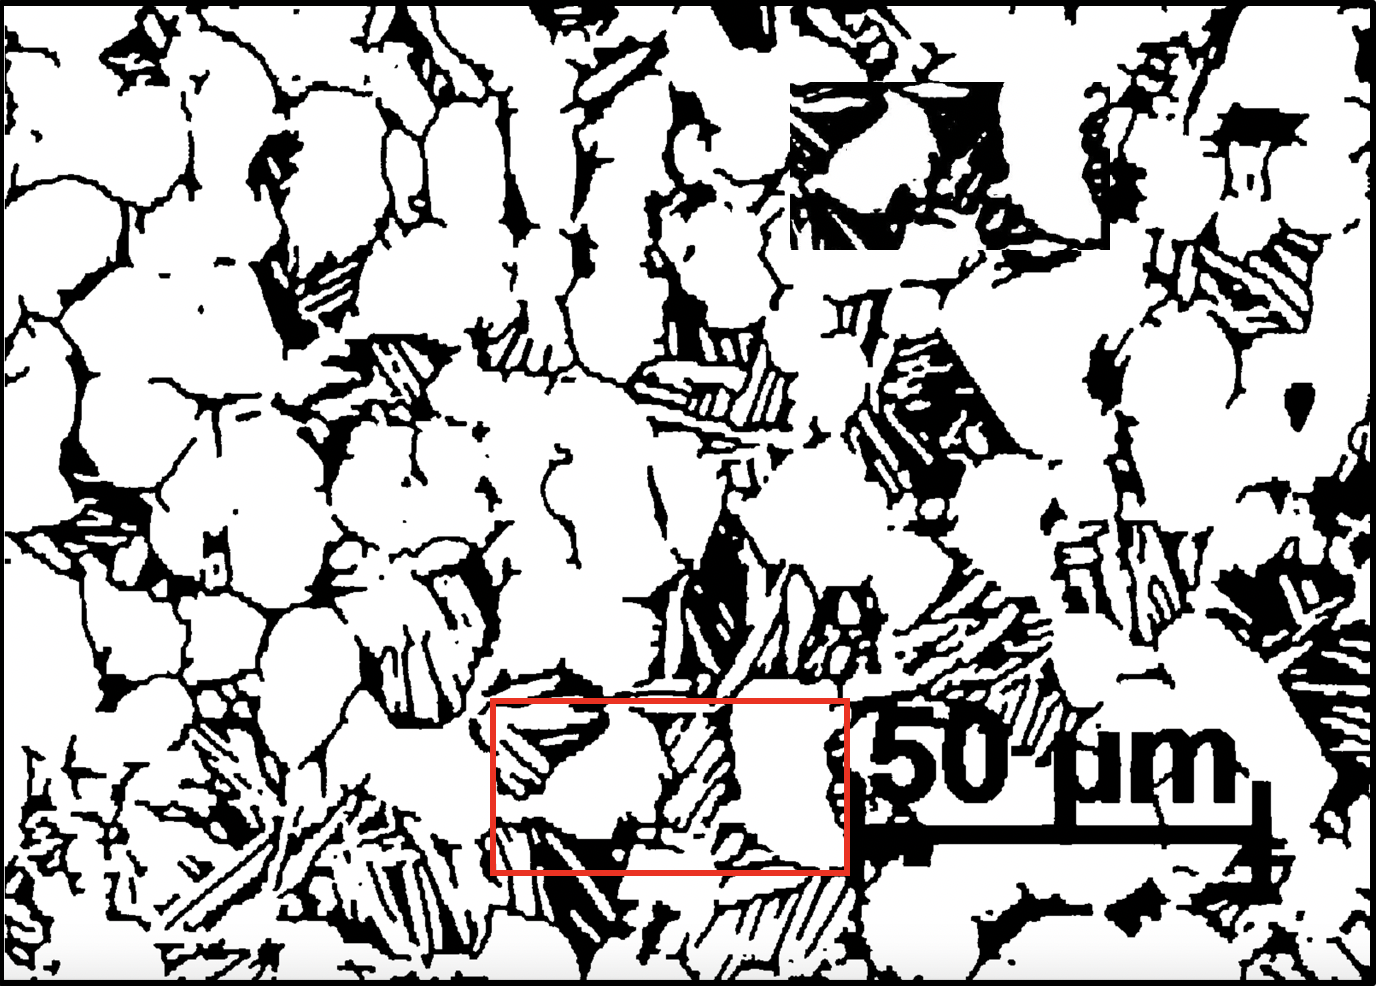
\includegraphics[width=13cm]{Ti64_Section_Taken.png}
    \caption{Image of globular Ti-6Al-4V which has been previously processed, showing the section (highlighted in red) for the FEM simulation}
    \label{fig:FinalSimulationInput}
\end{figure}
\\
The black (beta) and white (alpha) regions of the microstructure are considered to be separate materials within the simulation. The thermo-physical properties of the alpha and beta regions are assigned as specified in Table \ref{tab:Ti64Properties}. The microstructure skeleton is created using a 40x40 QuadSkeleton grid, which may include tri elements to gain greater accuracy despite the increarsed computational times. The skeleton is annealed, the edges are swapped and the skeleton smoothed to improve the homogeneity index to 0.940. The mesh is then generated from the skeleton, with the mapping and interpolation orders remain as 1 to save on computational time. The temperature and force fields are then defined on the mesh, constrained in-plane as active (such that the FE output contains the specified parameters). The boundary conditions for the temperature are set as 0 \degree C on the left edge and 1000 \degree C on the right edge. The force field boundary condition is fixed on the left edge, such that there is no (x,y) displacement on the edge. The solver tolerance is set to 1 x10$^-^1^3$ with 1000 iterations and the results are visualised. The stress contour map is created in post processing within the OOF2 program where the flux is set to stress and the invariant is set to trace.

\begin{center}
  \begin{table}[h!]
  \caption{\label{tab:Ti64Properties}Thermo-physical properties of the Ti-6Al-4V used in the heat diffusion simulation}
  \begin{center}
  \begin{tabular}{|p{6cm}|p{3cm}|p{3cm}|}
  \hline
  \textbf{Property} &\textbf{Alpha Phase} &\textbf{Beta Phase}\\
  \hline
  Young's Modulus, \textit{E} (GPa) & 92.8 & 75.8 \\
   \hline
   Poisson Ratio, $\nu$ & 0.35 & 0.31 \\
   \hline
   Thermal conductivity, $\kappa$ (W/mK) & 7.6 & 11.3 \\
   \hline
   Thermal expansion, $\alpha$ (x10$^-^6$ K$^-^1$) & 8.6 & 11.8 \\
   \hline  
  \end{tabular}
  \end{center}
  \end{table}
\end{center}

\end{document}
